\documentclass[UTF8,a4paper,11pt,fontset=fandol]{ctexart}
\newcommand{\DocTitle}{实验05：宠物主体分割与小型U-Net}
\newcommand{\DocSubject}{135分钟；PyTorch卷积编码器、语义分割、跳跃连接与107平台训练评估}
\newcommand{\DocShortTitle}{实验05：宠物主体分割}
\newcommand{\DocType}{学生讲义与实验手册}
% Shared style for integrated experiment handouts.
\usepackage[left=2.15cm,right=2.15cm,top=2.25cm,bottom=2.15cm,headsep=0.7cm]{geometry}
\usepackage{amsmath,amssymb}
\usepackage{booktabs,array,tabularx,longtable,multirow}
\usepackage{enumitem}
\usepackage{xcolor}
\usepackage{graphicx}
\usepackage{tikz}
\usetikzlibrary{arrows.meta,positioning,calc,shapes.geometric}
\usepackage{tcolorbox}
\usepackage{listings}
\usepackage{hyperref}
\usepackage{fancyhdr}
\usepackage{chngcntr}

\definecolor{Ink}{HTML}{17233C}
\definecolor{Navy}{HTML}{173B68}
\definecolor{Blue}{HTML}{2878B5}
\definecolor{Cyan}{HTML}{2A9D8F}
\definecolor{Amber}{HTML}{E9A23B}
\definecolor{Red}{HTML}{C84B4B}
\definecolor{Paper}{HTML}{F6F8FB}
\definecolor{PaleBlue}{HTML}{EAF2FA}
\definecolor{PaleCyan}{HTML}{EAF7F4}
\definecolor{PaleAmber}{HTML}{FFF5E4}
\definecolor{Rule}{HTML}{D6DEE8}
\definecolor{Muted}{HTML}{5B677A}

\hypersetup{
  colorlinks=true,
  linkcolor=Navy,
  urlcolor=Blue,
  citecolor=Cyan,
  pdfauthor={《人工智能数学原理与算法》课程组},
  pdftitle={\DocTitle},
  pdfsubject={\DocSubject}
}

\ctexset{
  section={format=\Large\bfseries\color{Navy},beforeskip=1.4ex plus .2ex,afterskip=.8ex},
  subsection={format=\large\bfseries\color{Ink},beforeskip=1.2ex plus .2ex,afterskip=.55ex},
  subsubsection={format=\normalsize\bfseries\color{Blue},beforeskip=1ex,afterskip=.35ex}
}

\setlength{\parindent}{2em}
\setlength{\parskip}{0.22em}
\setlength{\emergencystretch}{2em}
\linespread{1.14}
\setlist[itemize]{leftmargin=2em,itemsep=.25em,topsep=.35em}
\setlist[enumerate]{leftmargin=2.2em,itemsep=.28em,topsep=.35em}
\renewcommand{\arraystretch}{1.30}
\newcolumntype{Y}{>{\raggedright\arraybackslash}X}
\newcolumntype{C}[1]{>{\centering\arraybackslash}p{#1}}
\newcolumntype{L}[1]{>{\raggedright\arraybackslash}p{#1}}

\newcommand{\R}{\mathbb{R}}
\newcommand{\E}{\mathbb{E}}
\newcommand{\MSE}{\operatorname{MSE}}
\newcommand{\RMSE}{\operatorname{RMSE}}
\newcommand{\argmin}{\operatorname*{arg\,min}}
\newcommand{\vect}[1]{\boldsymbol{#1}}
\newcommand{\mat}[1]{\mathbf{#1}}
\newcommand{\term}[1]{\textcolor{Blue}{\textbf{#1}}}
\newcommand{\code}[1]{\texttt{#1}}
\numberwithin{equation}{subsection}

\tcbset{boxrule=.7pt,arc=1.6mm,left=2.5mm,right=2.5mm,top=1.8mm,bottom=1.8mm,before skip=7pt,after skip=7pt}
\newtcolorbox{keybox}[1][核心结论]{colback=PaleBlue,colframe=Blue,title={#1},fonttitle=\bfseries,coltitle=white}
\newtcolorbox{examplebox}[1][贯穿例题]{colback=PaleCyan,colframe=Cyan,title={#1},fonttitle=\bfseries,coltitle=white}
\newtcolorbox{questionbox}[1][检查点]{colback=PaleAmber,colframe=Amber,title={#1},fonttitle=\bfseries,coltitle=Ink}
\newtcolorbox{pitfallbox}[1][易错提醒]{colback=red!3,colframe=Red,title={#1},fonttitle=\bfseries,coltitle=white}
\newtcolorbox{teacherbox}[1][教师提示]{colback=Paper,colframe=Rule,title={#1},fonttitle=\bfseries,coltitle=Muted}
\newtcolorbox{proofbox}[1][推导与证明]{colback=Blue!3,colframe=Navy,title={#1},fonttitle=\bfseries,coltitle=white}

\lstdefinestyle{python}{
  language=Python,
  basicstyle=\ttfamily\small,
  keywordstyle=\color{Blue}\bfseries,
  commentstyle=\color{Cyan!70!black},
  stringstyle=\color{Red!80!black},
  showstringspaces=false,
  columns=fullflexible,
  keepspaces=true,
  frame=single,
  rulecolor=\color{Rule},
  backgroundcolor=\color{Paper},
  breaklines=true,
  numbers=left,
  numberstyle=\tiny\color{Muted},
  xleftmargin=1.5em,
  framexleftmargin=1.2em,
  aboveskip=.7em,
  belowskip=.7em
}
\lstset{style=python}

\pagestyle{fancy}
\fancyhf{}
\fancyhead[L]{\small\color{Muted}人工智能数学原理与算法}
\fancyhead[R]{\small\color{Muted}\DocShortTitle}
\fancyfoot[L]{\small\color{Muted}\DocType}
\fancyfoot[R]{\small\color{Muted}\thepage}
\renewcommand{\headrulewidth}{0pt}
\renewcommand{\footrulewidth}{0pt}

\newcommand{\makeexperimenttitle}[4]{
  \hypersetup{pageanchor=false}
  \begin{titlepage}\thispagestyle{empty}
  \begin{tikzpicture}[remember picture,overlay]
    \fill[Ink] (current page.north west) rectangle ([yshift=-9.4cm]current page.north east);
    \fill[Blue] ([yshift=-9.4cm]current page.north west) rectangle ([yshift=-9.68cm]current page.north east);
    \fill[Cyan] ([xshift=2.15cm,yshift=-1.55cm]current page.north west) rectangle ([xshift=2.27cm,yshift=-8.55cm]current page.north west);
    \fill[Paper] ([xshift=2.15cm,yshift=2.0cm]current page.south west) rectangle ([xshift=-2.15cm,yshift=6.15cm]current page.south east);
  \end{tikzpicture}
  \vspace*{1.45cm}
  {\color{white}\Large 人工智能数学原理与算法\par}\vspace{.55cm}
  {\color{white}\fontsize{31}{39}\selectfont\bfseries #1\par}\vspace{.35cm}
  {\color{white}\fontsize{21}{28}\selectfont #2\par}
  \vfill
  \begin{tcolorbox}[colback=white,colframe=white,boxrule=0pt,arc=0mm,left=7mm,right=7mm,top=6mm,bottom=6mm,width=\textwidth]
    \begin{tabularx}{\linewidth}{L{2.6cm}Y}
      \textcolor{Muted}{材料类型} & \DocType\\
      \textcolor{Muted}{实验安排} & #3\\
      \textcolor{Muted}{贯穿案例} & #4\\
      \textcolor{Muted}{适用对象} & 已完成机器学习导论、具备高中数学与基础计算机操作能力的本科生\\
    \end{tabularx}
  \end{tcolorbox}
  \vspace{.7cm}{\color{Muted}\small 版本：2026年秋季学期整合稿\hfill 源文件与 PDF 同目录交付\par}
  \end{titlepage}
  \hypersetup{pageanchor=true}
  \pagenumbering{roman}\tableofcontents\clearpage\pagenumbering{arabic}
}

\usepackage{xurl,bookmark}
\tcbuselibrary{breakable}
\setmonofont[BoldFont=DejaVuSansMono-Bold.ttf]{DejaVuSansMono.ttf}
\setCJKmonofont{FandolFang-Regular.otf}
\setlength{\headheight}{15pt}
\setcounter{tocdepth}{1}
\hypersetup{pdfauthor={钟志诚（主讲）；曾有成（整理）}}
\lstset{numbers=none,xleftmargin=0pt,framexleftmargin=0pt,basicstyle=\ttfamily\small}
\newcommand{\file}[1]{\nolinkurl{#1}}
\newcommand{\shape}[1]{\texttt{#1}}
\newcommand{\task}[1]{\textcolor{Blue}{\textbf{#1}}}
\begin{document}
\hypersetup{pageanchor=false}
\begin{titlepage}
\thispagestyle{empty}
\begin{tikzpicture}[remember picture,overlay]
\fill[Ink] (current page.north west) rectangle ([yshift=-10.1cm]current page.north east);
\fill[Cyan] ([yshift=-10.1cm]current page.north west) rectangle ([yshift=-10.28cm]current page.north east);
\end{tikzpicture}
\vspace*{1.0cm}
{\Large\color{white}人工智能数学原理与算法\par}
\vspace{1.0cm}
{\fontsize{34}{43}\selectfont\bfseries\color{white}实验05\par}
\vspace{.4cm}
{\fontsize{26}{34}\selectfont\bfseries\color{white}宠物主体分割\par}
\vspace{.3cm}
{\Large\color{white}从卷积编码器到小型 U-Net\par}
\vspace{.8cm}
{\large\color{Navy}学生讲义与实验手册\par}
\vspace{2.1cm}
\begin{tabular}{@{}ll}
主讲 & 钟志诚\\[.6em]
整理 & 曾有成\\[.6em]
单位 & 中国科学技术大学\\
 & 人工智能与数据科学学院
\end{tabular}
\vspace{1cm}
\begin{keybox}[本次实验要完成的作品]
输入一张宠物照片，输出主体区域。自己搭建卷积编码器，接入提供的解码器，在学校107平台训练和评估，再用跳跃连接改进细节恢复。
\end{keybox}
\vfill
2026年秋季\quad 3学时（135分钟），完整训练与对比可课后完成。\\
框架：PyTorch\quad 数据：Oxford-IIIT Pet\quad 不需要Kaggle账号。
\end{titlepage}
\hypersetup{pageanchor=true}
\pagenumbering{roman}
\tableofcontents
\vfill
\begin{teacherbox}[阅读顺序]
先完成第1--8节的基础任务；第9--11节为进阶与改进提示。首次阅读只需看懂每一步的输入、操作和输出，随后用检查程序核对。源代码中的 TODO 表示待补全位置，Hint 表示提示。
\end{teacherbox}
\clearpage\pagenumbering{arabic}

\section{实验目标与课堂安排}
\subsection{从分类走向逐像素预测}
正课已经介绍 CNN（Convolutional Neural Network，卷积神经网络）的局部连接、权重共享、池化与残差连接。本实验把这些结论用于一个具体任务：从照片中找出宠物主体。分类只给整张图一个类别；\term{语义分割}要给每个像素一个类别。本实验只区分宠物和背景，不识别品种，也不区分多只宠物的个体。

完成实验后，应能：解释卷积、激活与池化的作用；填写各层尺寸和参数量；自己搭建编码器；在固定划分上完成模型选择；解释分割误差；比较 U-Net 拼接与 ResNet（Residual Network，残差网络）的相加连接。
\subsection{任务边界与分工}
\par\noindent\begin{tabularx}{\linewidth}{L{2.4cm}YY}\toprule
部分 & 学生完成 & 已提供\\\midrule
基础运算 & 小矩阵卷积、激活、池化 & 可运行示例与自检\\
网络 & 基础和改进编码器 & 基础解码器、训练程序\\
数据与评价 & 观察样本、解释指标 & 数据划分、掩码转换、指标实现\\
平台与分析 & 提交作业、对比、报告 & 提交脚本、日志和报告模板\\
进阶（选做） & 自行实现小型 U-Net 并接入训练 & 结构示意和维度提示，不提供代码骨架\\\bottomrule
\end{tabularx}\par
\subsection{135分钟课堂流程}
\par\noindent\begin{tabularx}{\linewidth}{L{1.5cm}L{1.6cm}YY}\toprule
时间 & 任务 & 教师活动 & 学生活动与可观察产出\\\midrule
0--15 & T1 & 解释任务和三值标注 & 查看样本，说出忽略区域\\
15--35 & T2 & 演示一次滑窗计算 & 完成手算与三个小函数\\
35--55 & T3前半 & 解释通道与尺寸 & 搭建阶段1，核对输出\\
55--70 & T3后半 & 指导阶段连接 & 完成三阶段尺寸表\\
70--90 & T4 & 解释损失与更新 & 检查完整网络和一次更新\\
90--115 & T5 & 演示107作业提交 & 提交短任务，读日志\\
115--135 & T6/进阶 & 讲解结果分析与拼接 & 完成对比计划和退出卡\\\bottomrule
\end{tabularx}\par
净教学时间合计135分钟；安装、下载和排队不计入其中。课堂先接通网络，完整训练和第二组实验可课后完成。
\clearpage

\section{T1：数据、标注与划分}
\subsection{同一张图的三个角色}
Oxford-IIIT Pet 数据由牛津大学等团队发布，包含猫狗照片与像素级三值标注（trimap）。\term{掩码}是与图片空间位置对应的标签数组。输入使用 RGB（Red, Green, Blue，红绿蓝）三通道，统一缩放为128$\times$128。
\par\noindent\begin{tabularx}{\linewidth}{L{2cm}L{3cm}YY}\toprule
原始像素值 & 原始含义 & 训练目标 & 有效区域\\\midrule
1 & 宠物前景 & 1 & 1\\
2 & 背景 & 0 & 1\\
3 & 未确定区域 & 占位为0 & 0：不计损失与指标\\\bottomrule
\end{tabularx}\par
“目标为0、有效区域为0”不表示把边界训练成背景。它表示这个位置不参与当前目标。程序中的\file{target}和\file{valid}必须配合使用。
\begin{center}
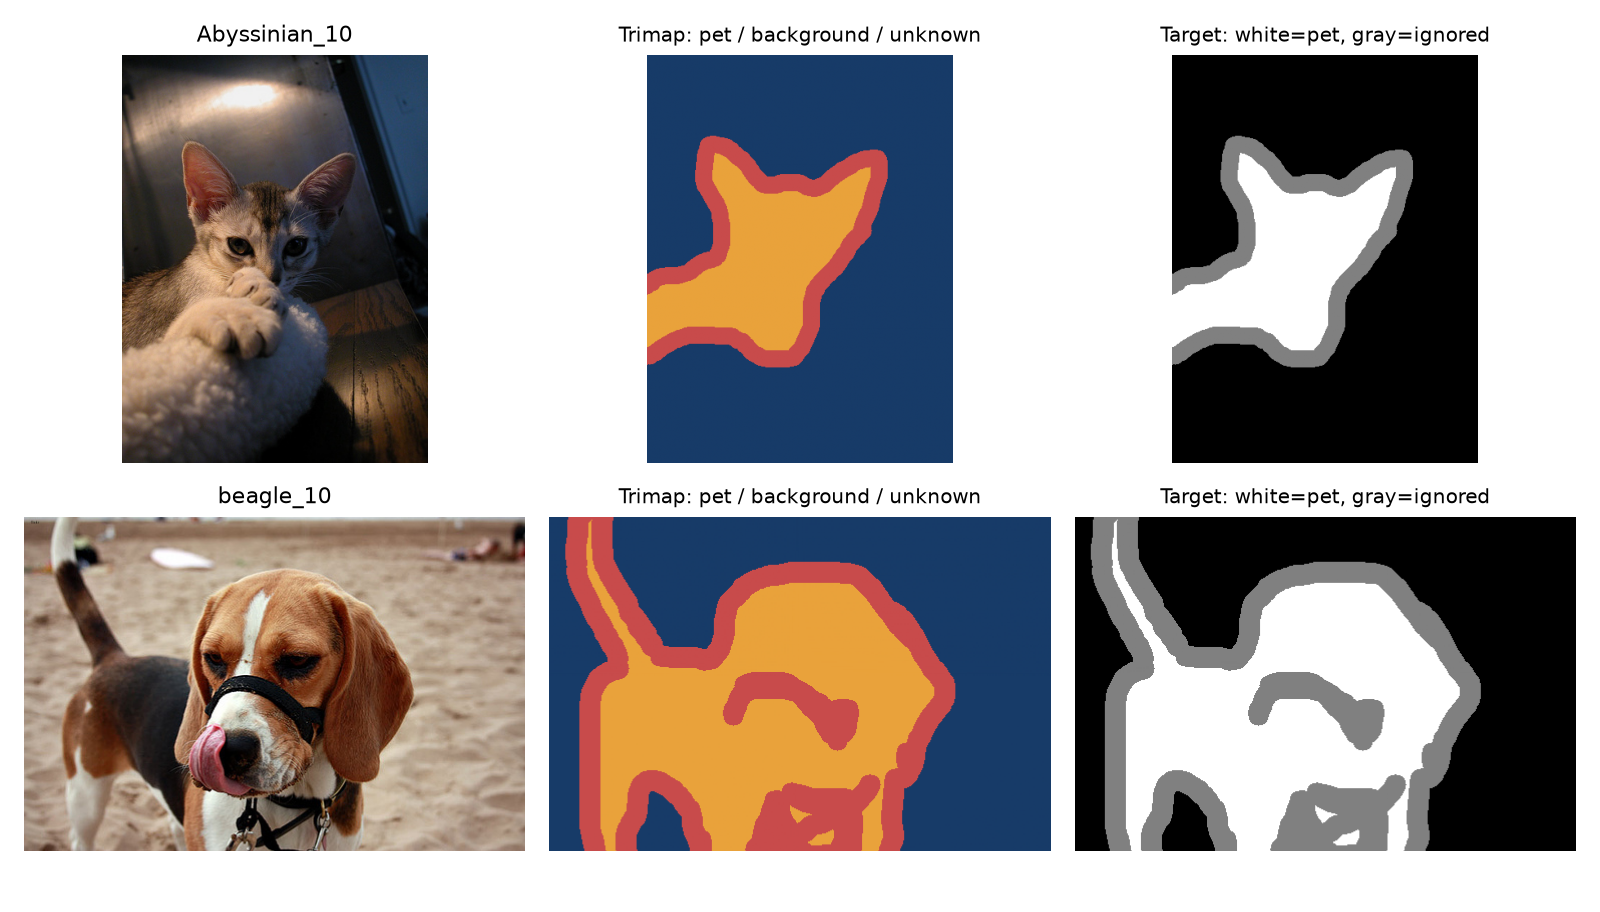
\includegraphics[width=.84\linewidth]{assets/pet-data.png}
\end{center}
上图来自官方训练划分中的样本。左为图片，中为原始标注（橙色宠物、深蓝背景、红色未确定），右为本实验使用的目标；右图白色为宠物、黑色为背景、灰色为忽略区域。图中的空间对齐是监督信号成立的前提。
\subsection{划分与变换}
保留官方测试集；只在官方 \file{trainval.txt} 名单内按品种分组，使用固定种子2026划分80\%训练、20\%验证（每类训练数量向下取整）。\file{splits.json}保存明确名单，运行记录保存其指纹。生成后为2941张训练、739张验证、3669张测试。它与控制网络初始化的训练种子42用途不同。

图片用双线性插值缩放；标签用最近邻插值，避免产生不存在的类别值。若启用水平翻转，图片和掩码必须一起翻转；验证与测试不使用随机变换。固定缩放可能改变原图长宽比例，这是本教学协议的局限，所有模型采用同一规则。
\begin{questionbox}[检查点]
如果只翻转图片而不翻转掩码，会发生什么？如果把值3直接送进二元损失，又错在哪里？先解释再运行 \file{preview_data.py}。
\end{questionbox}
\clearpage

\section{T2：卷积、激活与池化怎样执行}
\subsection{卷积核是可学习的局部计算规则}
邱锡鹏《神经网络与深度学习》第5章用局部连接和权重共享解释卷积层。本实验沿用该概念，但层号使用下标，样本编号使用括号上标。为便于手算，本页使用自编单通道矩阵，不冒充教材数据。

设输入矩阵为$\mathbf X\in\mathbb R^{3\times3}$，卷积核为$\mathbf K\in\mathbb R^{2\times2}$，偏置为0，步长为1且不填充：
\begin{equation}
\mathbf X=\begin{bmatrix}1&2&3\\4&5&6\\7&8&9\end{bmatrix},\qquad
\mathbf K=\begin{bmatrix}1&0\\0&-1\end{bmatrix}.
\end{equation}
卷积核在输入上移动，每次对齐窗口内的元素，逐元素相乘再求和。PyTorch的\file{Conv2d}实际执行不翻转核的互相关，课程中仍习惯称其为卷积。左上角输出为：
\begin{equation}
z_{11}=1\times1+2\times0+4\times0+5\times(-1)=-4.
\end{equation}
这里$z_{11}$是激活前得分矩阵$\mathbf Z$的第1行第1列。向右、向下重复同一组权重，得到
\begin{equation}
\mathbf Z=\begin{bmatrix}-4&-4\\-4&-4\end{bmatrix}.
\end{equation}
\subsection{把公式变成循环}
先运行\file{python operator_exercises.py}查看完整的PyTorch例子，再补全\file{correlate2d}。本练习只实现二维、步长1、无填充；完整网络使用PyTorch基础层及自动求导。
\begin{lstlisting}
window = image[row:row+kh, col:col+kw]
# Hint: multiply corresponding entries, then sum.
\end{lstlisting}
\begin{questionbox}[修改一个值]
把$\mathbf X$中心的5改为10。四个输出是否都会改变？先看中心像素在各窗口中对应哪个核元素，再运行程序检查。
\end{questionbox}
\begin{pitfallbox}
卷积层不是对每个位置学习一套核；同一个输出通道的核在空间位置之间共享。窗口内的点积也不是普通矩阵乘法。
\end{pitfallbox}
\clearpage

\subsection{激活改变数值，池化改变空间尺寸}
ReLU（Rectified Linear Unit，修正线性单元）对每个元素计算$g(z)=\max(0,z)$，输入和输出形状相同。负数变成0，正数保留；它为多层网络引入非线性。上一页的$\mathbf Z$经ReLU后全为0。这个核对此输入没有产生正响应，不表示所有卷积核都无效。

最大池化（邱书称最大汇聚）从局部窗口选最大值。对自编激活矩阵$\mathbf A\in\mathbb R^{4\times4}$使用2$\times$2窗口、步长2：
\begin{equation}
\mathbf A=\begin{bmatrix}1&3&2&0\\4&2&1&5\\0&6&3&1\\2&1&4&2\end{bmatrix}
\quad\longrightarrow\quad
\begin{bmatrix}4&5\\6&4\end{bmatrix}.
\end{equation}
每个输入通道独立池化，通道数不变。池化没有可训练的卷积权重；它降低计算量，也舍弃部分位置细节。\task{补全T2.2与T2.3后运行：}
\begin{lstlisting}[language=bash]
python checks.py operators
\end{lstlisting}
\subsection{先算尺寸，再写代码}
高度方向的输入、输出尺寸分别为$H_{\mathrm{in}}$和$H_{\mathrm{out}}$；卷积核大小为$k$，两侧填充各$p$个像素，步长为$s$。本实验膨胀率固定为1：
\begin{equation}
H_{\mathrm{out}}=\left\lfloor\frac{H_{\mathrm{in}}+2p-k}{s}\right\rfloor+1.
\end{equation}
$\lfloor\cdot\rfloor$表示向下取整；宽度方向同理。128像素输入经过$k=3,p=1,s=1$卷积仍为128，再经过$k=2,p=0,s=2$池化变为64。

若输入通道数为$C_{\mathrm{in}}$、输出通道数为$C_{\mathrm{out}}$，普通二维卷积的参数量（包含每个输出通道的偏置）为：
\begin{equation}
P=C_{\mathrm{out}}(C_{\mathrm{in}}k^2+1).
\end{equation}
例如3通道到16通道、3$\times$3卷积有$16(3\times9+1)=448$个参数。空间分辨率不出现在该式中，这体现了权重共享。
\begin{questionbox}[检查点]
3$\times$3卷积把16通道变为32通道，参数量是多少？池化后通道数是否减半？把答案填入报告。
\end{questionbox}
\clearpage

\section{T3：自己搭建编码器}
\subsection{读懂四维张量}
张量是多维数组。PyTorch图像批量采用\shape{[B,C,H,W]}顺序：$B$为本批图片数，$C$为通道数，$H,W$为高、宽。样本位于第0维，原图的三个通道对应红绿蓝；中间特征的通道由网络学习，不再直接等于颜色。

\file{PetEncoder}继承\file{nn.Module}。在\file{__init__}里创建层，使参数被注册；在\file{forward}里按顺序调用层。不要在每次\file{forward}时重新创建卷积，否则新权重不能按预期持续学习。
\subsection{三阶段固定接口}
\par\noindent\begin{tabularx}{\linewidth}{L{2.1cm}L{4.2cm}Y}\toprule
位置 & 形状 & 你需要保证的事情\\\midrule
输入 & \shape{[B,3,128,128]} & 保留空间结构\\
\file{e1} & \shape{[B,16,64,64]} & 阶段1后空间减半\\
\file{e2} & \shape{[B,32,32,32]} & 输入通道匹配上一阶段\\
\file{z} & \shape{[B,64,16,16]} & 最深层特征仍为四维\\\bottomrule
\end{tabularx}\par
\file{z}只是代码中最深层特征的变量名；正文的数学$z$在损失部分专指输出头的激活前得分，请按上下文区分。

\task{T3.1--T3.3：}在\file{student_encoder.py}中用\file{nn.Sequential}组织卷积、ReLU、池化。\task{T3.4：}依次计算并返回\file{e1,e2,z}。示例语法如下；这里的$C$等符号是占位提示，不能原样运行：
\begin{lstlisting}
nn.Conv2d(in_channels, out_channels, kernel_size=3,
          stride=1, padding=1)
nn.ReLU()
nn.MaxPool2d(kernel_size=2, stride=2)
\end{lstlisting}
\begin{lstlisting}[language=bash]
python checks.py encoder
python checks.py basic
\end{lstlisting}
检查程序会打印三个阶段的尺寸，再检查梯度和一次更新。未完成的骨架使用\file{Identity}占位，它能导入，但不会假装通过任务。
\begin{pitfallbox}[最常见的连接错误]
上一层输出16通道，下一层却写\file{Conv2d(3,32,...)}；忘记池化；池化重复两次；展平后丢失空间维。遇到错误先打印\file{x.shape}，再检查输入通道和空间尺寸。
\end{pitfallbox}
\clearpage

\section{T4：连接提供的解码器}
\subsection{编码器和解码器分别负责什么}
编码器把局部像素变成更抽象、分辨率更低的特征；解码器把这些特征转成逐像素输出。这里的backbone指承担主要特征提取的编码器。基础模型只使用最深层特征，不使用中间层的跳跃连接。
\begin{center}
\begin{tikzpicture}[node distance=6mm,every node/.style={font=\small},box/.style={draw=Blue,fill=PaleBlue,rounded corners,minimum width=11cm,minimum height=9mm,align=center},arr/.style={-Latex,thick,Navy}]
\node[box] (a) {图片：$B\times3\times128\times128$};
\node[box,below=of a] (b) {学生编码器：$128\rightarrow64\rightarrow32\rightarrow16$};
\node[box,below=of b] (c) {最深层特征：$B\times64\times16\times16$};
\node[box,below=of c,fill=PaleCyan,draw=Cyan] (d) {提供的解码器：$16\rightarrow32\rightarrow64\rightarrow128$};
\node[box,below=of d,fill=PaleCyan,draw=Cyan] (e) {像素得分：$B\times1\times128\times128$};
\draw[arr] (a)--(b);\draw[arr] (b)--(c);\draw[arr] (c)--(d);\draw[arr] (d)--(e);
\end{tikzpicture}
\end{center}
蓝色框表示学生负责的编码路径，青色框表示提供的解码路径；箭头表示数据流。框中的空间尺寸变化不表示通道数同步变化。
\subsection{上采样与输出头}
\file{ProvidedDecoder}使用双线性上采样加卷积，每次扩大空间尺寸后学习特征组合。最后一个1$\times$1卷积把16个通道组合成1个像素得分。
\begin{lstlisting}
x = F.interpolate(features, scale_factor=2,
                  mode="bilinear", align_corners=False)
x = self.block2(x)
\end{lstlisting}
插值不含可训练权重，只根据邻近位置计算新值。它能放大特征图，却不能凭空恢复已经丢弃的信息。后续卷积的参数通过标注学习，跳跃连接则提供另一条细节信息来源。
\begin{questionbox}[检查点]
最终输出为什么是1个通道而不是2个？答案是本实验用一个得分表示“属于宠物”的概率；背景概率由1减去该概率得到。二通道建模也可行，但损失和标签接口不同，本实验保持统一。
\end{questionbox}
\clearpage

\section{损失、梯度与分割指标}
\subsection{从像素标签得到训练目标}
对第$n$张图片的第$u$个空间位置，$y_u^{(n)}\in\{0,1\}$表示背景或宠物，$m_u^{(n)}\in\{0,1\}$表示是否有效。$z_u^{(n)}\in\mathbb R$是网络输出的原始得分，$p_u^{(n)}$是宠物概率。sigmoid函数把实数映射到$(0,1)$：
\begin{equation}
p_u^{(n)}=\sigma(z_u^{(n)})=\frac{1}{1+\exp(-z_u^{(n)})}.
\end{equation}
$\exp$是自然指数函数。把每个有效像素视为一个伯努利标签预测问题，负对数似然给出\term{二元交叉熵}。这是逐像素的训练模型，不表示真实图像中的像素相互独立。
\begin{equation}
\mathcal L_{\mathrm{pix}}(z,y)=-y\log\sigma(z)-(1-y)\log(1-\sigma(z)).
\end{equation}
$\log$为自然对数；$\mathcal L_{\mathrm{pix}}$为局部像素损失，整张图和批量损失仍统一使用$\mathcal L$。设$M^{(n)}=\sum_u m_u^{(n)}$为有效像素数，则
\begin{equation}
\mathcal L^{(n)}=\frac{\sum_u m_u^{(n)}\mathcal L_{\mathrm{pix}}(z_u^{(n)},y_u^{(n)})}{M^{(n)}},\qquad
\mathcal L_B=\frac1B\sum_{n=1}^{B}\mathcal L^{(n)}.
\end{equation}
这里$\sum$表示求和。分母按每张图的有效像素数计算，使图片在批量中等权。代码用分母至少为1处理全忽略的调试输入，此时损失贡献为0。
\subsection{一次可核对的更新}
偏导符号$\partial$描述改变一个变量时函数的变化率。记$p=\sigma(z)$，则$\mathrm dp/\mathrm dz=p(1-p)$。由链式法则得到
\begin{equation}
\frac{\partial\mathcal L_{\mathrm{pix}}}{\partial z}
=\left(-\frac yp+\frac{1-y}{1-p}\right)p(1-p)=p-y.
\end{equation}
乘上有效掩码后，忽略位置的梯度为0。若一张教学小图只有两个有效像素，标签为$[1,0]$，得分为$[0,0]$，则概率为$[0.5,0.5]$，平均损失为$\log2\approx0.6931$。把两个得分写成向量$\mathbf z\in\mathbb R^2$，对它的梯度为
\begin{equation}
\frac{\partial\mathcal L}{\partial\mathbf z}
=\frac12[0.5-1,\;0.5-0]=[-0.25,\;0.25].
\end{equation}
把这两个得分暂当可直接更新的变量，学习率$\eta=0.1$时，一步梯度下降得到$[0.025,-0.025]$。真实网络更新的是产生得分的参数，通过链式法则传递梯度；这个小例子只用于解释方向。
\begin{pitfallbox}
\file{binary_cross_entropy_with_logits}已包含数值稳定的sigmoid处理。模型末尾不要先做sigmoid再把概率传给它。
\end{pitfallbox}
\clearpage

\subsection{为什么不只看像素准确率}
如果背景占90\%，全预测背景也有90\%像素准确率，但没有找到宠物。我们主要评价前景区域的重合程度。在有效区域内，设$P$是预测宠物像素集合，$G$是真实宠物像素集合，$|P|$表示集合中的像素个数：
\begin{equation}
\mathrm{IoU}=\frac{|P\cap G|}{|P\cup G|},\qquad
\mathrm{Dice}=\frac{2|P\cap G|}{|P|+|G|}.
\end{equation}
IoU（Intersection over Union）为交并比；$\cap$取共有像素，$\cup$取至少属于一个集合的像素。Dice为另一种重合系数，二者越大越好。预测使用$p\geq0.5$，等价于原始得分$z\geq0$。
\begin{examplebox}[手算评价]
预测前景有3个像素，真实前景也有3个，其中2个重合。并集有$3+3-2=4$个，因此IoU为$2/4=0.5$，Dice为$4/6\approx0.6667$。若另有一个忽略位置被预测为前景，它不改变这两个结果。
\end{examplebox}
\subsection{统一评价口径}
\begin{itemize}
\item 在缩放后的128$\times$128标签网格上计算；不在原图尺寸上另算一套成绩。
\item 先排除原始标签为3的位置，再计算每张图的前景IoU和Dice。
\item 对所有图片取算术平均，不能先合并所有像素，也不能直接平均大小不同的批次。
\item 双方前景都为空时记1；只有一方为空时记0。真实宠物数据正常应有前景，全忽略输入只用于程序边界检查。
\item 主指标为平均前景IoU，辅助指标为平均Dice。不要把它称为“前景与背景两类的平均IoU”。
\end{itemize}
\subsection{训练、验证和测试的职责}
训练集用于反向传播；每轮在验证集上计算指标，保存验证IoU最高的轮次（并列保留较早轮次）。根据验证结果选择网络和超参数后，才对选定模型执行最终测试。不要从测试分数反复返回修改模型。
\begin{lstlisting}[language=bash]
python checks.py core
\end{lstlisting}
这个自检不依赖学生网络，检查标签转换、边界梯度、手算指标及空前景情况。若它失败，应先检查提供代码和环境，而不是继续训练。
\clearpage

\section{运行准备与本地调试}
\subsection{环境与数据}
沿用实验04验证过的Python环境。参考依赖为Python 3.11、PyTorch 2.7.1、Torchvision 0.22.1；具体计算设备支持以安装的构建版本为准。CPU（Central Processing Unit，中央处理器）可完成前向和短流程检查，正式实验使用GPU（Graphics Processing Unit，图形处理器）。进入\file{code/}后运行：
\begin{lstlisting}[language=bash]
python -m pip install -r requirements.txt
python checks.py core
python checks.py demo
python prepare_data.py --data-dir data --download
python preview_data.py --data-dir data
\end{lstlisting}
在联网机器上下载一次，再将数据上传到平台。若环境已配好，无需重复安装。GPU版PyTorch需要与驱动兼容；安装方式沿用实验04核对过的方案，不能用安装成功代替设备可用性检查。
\begin{lstlisting}
data/
  splits.json
  oxford-iiit-pet/
    images/
    annotations/
      trainval.txt
      test.txt
      trimaps/
\end{lstlisting}
\subsection{先运行一个完整的小例子}
\file{demo}是已完成的极简网络；\file{--synthetic}生成带圆形前景的合成图。两者用于在TODO未完成时检查程序，不作为宠物分割成绩。
\begin{lstlisting}[language=bash]
python train.py --model demo --synthetic --device cpu \
  --epochs 1 --limit-train 8 --limit-val 4 \
  --output outputs/demo-local
\end{lstlisting}
以上反斜线续行用于平台的Bash终端。在Windows PowerShell中应合并为一行执行。运行会生成\file{run.json}、\file{history.csv}、\file{best.pt}和图片。改一个学习率或输入值，观察输出，再补全学生函数。
\begin{questionbox}[检查点]
为什么合成图上的高分不能写成宠物分割效果？为什么\file{demo}能运行不代表T3编码器已经完成？
\end{questionbox}
\clearpage

\section{T5：在107平台训练与记录}
\subsection{从短作业开始}
上传完整\file{code/}和数据目录，在107平台登录／提交终端进入\file{code/}。先设置实验04已核对的环境解释器路径；以下环境名为示例：
\begin{lstlisting}[language=bash]
export LAB05_PYTHON="$HOME/.conda/envs/compute-resnet/bin/python"
export LAB05_DATA_DIR="$PWD/data"
bash scripts/submit.sh smoke
squeue -u "$USER"
\end{lstlisting}
\file{smoke}运行合成短任务。日志必须显示CUDA（Compute Unified Device Architecture）设备和GPU名称。程序显式要求GPU，失败时不自动切到CPU。\file{Students}分区及QOS（Quality of Service，服务质量）\file{qos_stu_default}沿用实验04候选设置，按当前账号权限核对。
\subsection{提交基础与改进实验}
\begin{lstlisting}[language=bash]
export LAB05_EPOCHS=20
export LAB05_BATCH_SIZE=16
export LAB05_LR=0.001
export LAB05_SEED=42
bash scripts/submit.sh basic
bash scripts/submit.sh improved
\end{lstlisting}
先完成对应自检，再提交正式作业。默认申请单卡、4个CPU核心、8GB主内存和1小时；1小时是候选申请时限，不是实测训练时长。可在\file{submit.sh}末尾追加平台允许的\file{sbatch}资源选项，例如\file{--time=02:00:00}。

输出位于\textrm{outputs/模型名-作业号/}，日志位于\file{logs/}。用\textrm{tail -f logs/实际日志名.out}观察进度，使用\textrm{scancel 作业号}取消自己不再需要的作业。不要在登录节点直接启动长训练。
\subsection{训练程序的关键顺序}
\begin{lstlisting}
model.train()
optimizer.zero_grad()
logits = model(images)
loss = masked_loss(logits, targets, valid)
loss.backward()
optimizer.step()
\end{lstlisting}
验证使用\file{model.eval()}与\file{torch.no_grad()}。前者切换模块行为，后者停止构建梯度图，二者不能相互代替。每轮记录训练损失和验证损失、IoU、Dice，不自动评估测试集。
\clearpage

\section{进阶选做：自行实现小型U-Net}
\subsection{把浅层细节送回解码器}
基础解码器只收到16$\times$16特征。U-Net增加编码器到解码器的跨层连接，让解码器同时看到深层表示和相对精细的空间特征。本实验为两条跳跃连接的教学简化版；没有原论文的完整深度，也没有全分辨率跳跃连接。
\begin{center}
\begin{tikzpicture}[every node/.style={font=\small},box/.style={draw=Blue,fill=PaleBlue,rounded corners,minimum width=3.1cm,minimum height=1cm,align=center},arr/.style={-Latex,thick,Navy},skip/.style={-Latex,thick,Cyan}]
\node[box] (e1) at (0,0) {编码特征e1\\$16\times64\times64$};
\node[box] (e2) at (0,-1.8) {编码特征e2\\$32\times32\times32$};
\node[box] (z) at (0,-3.6) {深层特征z\\$64\times16\times16$};
\node[box,fill=PaleCyan,draw=Cyan] (d2) at (7,-1.8) {融合d2\\$32\times32\times32$};
\node[box,fill=PaleCyan,draw=Cyan] (d1) at (7,0) {融合d1\\$16\times64\times64$};
\draw[arr] (e1)--(e2);\draw[arr] (e2)--(z);
\draw[arr] (z.east)-|node[below,pos=.25]{上采样} (d2.south);
\draw[arr] (d2)--node[right]{上采样} (d1);
\draw[skip] (e2)--node[above]{拼接：$64+32$通道} (d2);
\draw[skip] (e1)--node[above]{拼接：$32+16$通道} (d1);
\end{tikzpicture}
\end{center}
图中省略批量维，青色横箭头为跳跃连接，深色箭头为顺序路径。d1再上采样至128$\times$128，自行设计输出头产生单通道得分。学生包仅提供基础编码器--解码器骨架，本节为独立选做，不附U-Net代码文件或现成运行入口。
\subsection{实现步骤与维度提示}
\par\noindent\begin{tabularx}{\linewidth}{L{1.4cm}YY}\toprule
步骤 & 自行实现 & Hint\\\midrule
1 & 第一次融合卷积 & 拼接后96通道，卷积输出32通道\\
2 & 第二次融合卷积 & 拼接后48通道，卷积输出16通道\\
3 & 第一处融合 & \file{torch.cat([up2,e2],dim=1)}后调用融合块\\
4 & 第二处融合 & 空间对齐后拼接\file{up1}与\file{e1}\\\bottomrule
\end{tabularx}\par
\file{F.interpolate(...,size=skip.shape[-2:])}明确对齐高和宽；\file{dim=1}沿通道拼接。保持最终输出为\shape{[B,1,128,128]}，继续使用同一损失与指标。
建议另建模型文件，自行扩展\file{models.py}的\file{build_model}、\file{train.py}的模型选项及\file{checks.py}的检查入口；再复制并调整平台脚本的训练分支。先核对输出形状、有限损失与参数更新，再做合成短训练、保存恢复和真实数据实验。基础任务不需要这些扩展。
\clearpage

\section{联系ResNet：跳跃连接怎样组合特征}
\subsection{相加与拼接的共同点和区别}
两者都让信息通过跨层路径传播，但组合方式不同。残差相加为优化提供较直接的路径；U-Net拼接保留两组通道，供后续卷积学习如何融合。不能把它们简单视为同一个运算。

设输入特征张量$\mathbf X\in\mathbb R^{B\times C\times H\times W}$，$F$是若干层组成的可学习变换，输出形状与输入相同。残差块的相加为
\begin{equation}
\mathbf Y=F(\mathbf X)+\mathbf X.
\end{equation}
它逐元素相加，通常要求四个维度都一致；不要靠广播凑形状。若通道或步长不同，可对捷径使用1$\times$1投影卷积，使其与主支路匹配。

U-Net中设上采样特征$\mathbf U\in\mathbb R^{B\times C_u\times H\times W}$、跳跃特征$\mathbf E\in\mathbb R^{B\times C_e\times H\times W}$。沿通道拼接得到
\begin{equation}
\mathbf C=\operatorname{Concat}_{\mathrm{channel}}(\mathbf U,\mathbf E)
\in\mathbb R^{B\times(C_u+C_e)\times H\times W}.
\end{equation}
$\operatorname{Concat}$表示连接数组；输入通道可以不同，但批量、高、宽应相同。随后卷积的\file{in_channels}必须使用相加后的通道数。
\par\noindent\begin{tabularx}{\linewidth}{L{2.6cm}YY}\toprule
比较项 & 残差相加 & U-Net通道拼接\\\midrule
代码形式 & \file{main + shortcut} & \file{torch.cat(...,dim=1)}\\
输出通道 & 保持匹配后的通道数 & 两支通道数之和\\
关注点 & 学习相对输入的修正 & 融合不同层的表示与细节\\\bottomrule
\end{tabularx}\par
\subsection{选做：让融合块带残差}
在完成U-Net后，可把融合卷积块改为残差块。先用1$\times$1卷积把96通道映射到32通道，再在32通道上做残差变换。不要直接把96通道张量与32通道张量相加。实验时只改变融合块，记录参数量和相同预算下的验证指标。
\begin{questionbox}[检查点]
两个张量都是\shape{[B,32,32,32]}，相加与拼接分别得到什么形状？如果一支为64通道，哪种操作可直接进行？
\end{questionbox}
\clearpage

\section{改进提示：归一化与泛化}
\subsection{批量归一化的使用位置}
BN（Batch Normalization，批量归一化）可帮助训练；是否提高验证表现需要对照实验。对\shape{[B,C,H,W]}特征，\file{BatchNorm2d(C)}在训练时对每个通道汇总批量和空间位置的统计量，随后使用可学习的缩放和平移。
\begin{lstlisting}
nn.Conv2d(16, 32, 3, padding=1)
nn.BatchNorm2d(32)
nn.ReLU()
\end{lstlisting}
以上是按顺序放入\file{nn.Sequential}的层。默认设置下，\file{train()}使用当前批次统计量并更新运行统计；\file{eval()}使用运行统计。批量很小、样本相关性高或训练测试分布不同，都可能影响效果。每通道还包含缩放$\gamma$和平移$\beta$两个可训练参数，参数统计要计入它们。
\subsection{层归一化必须说清维度}
LN（Layer Normalization，层归一化）按指定的最后若干维归一化，不使用跨样本的批统计量；训练和评估均使用当前输入统计量。PyTorch的\file{normalized_shape}决定归一化范围。
\begin{itemize}
\item \file{LayerNorm([C,H,W])}：对每张图该层的全部通道与空间位置归一化；形状固定，默认仿射参数也是$C\times H\times W$个缩放和同样多的平移，需关注参数量。
\item \file{LayerNorm(C)}：只处理最后一维。如果希望对每个像素的通道向量归一化，先把通道移到最后，再移回。这个范围与上一种不同，应在报告中说明。
\end{itemize}
\begin{lstlisting}
# In __init__: self.norm = nn.LayerNorm(channels)
# In forward, x has shape [B,C,H,W]:
x = x.permute(0, 2, 3, 1)    # [B,H,W,C]
x = self.norm(x)
x = x.permute(0, 3, 1, 2)    # [B,C,H,W]
\end{lstlisting}
\begin{pitfallbox}
不要直接在\shape{[B,C,H,W]}上套\file{LayerNorm(C)}。它可能因维度不匹配而报错；若宽度恰好等于C，还可能悄悄沿错误的轴计算。
\end{pitfallbox}
\subsection{怎样证明你的改动有帮助}
先保留基础版，再在\file{ImprovedEncoder}中只改一个主要因素。固定划分、输入分辨率、训练种子、轮数、批量大小与学习率，比较验证IoU、损失曲线和参数量。若加入数据增强，应作为另一组独立实验。泛化是对未参与训练的数据表现更好，训练损失下降本身不能证明泛化改善。
\clearpage

\section{T6：对比、评分与最终提交}
\subsection{至少两组实验}
基础要求为一个基线和一个改进编码器，使用同一提供的解码器。进阶选做U-Net，由学生自行编写，不提供代码骨架。默认参考预算为20轮、批量16、学习率0.001，正式时长由平台预跑确认；因显存调整批量时，应同步调整对照组并记录。

在验证样例中选至少3个成功和3个失败案例，观察耳朵、腿、毛发边缘、相似背景和小目标。既看分数，也看网络把什么当成了宠物。没有提升也要保留结果，解释可能原因，不要求每次改动都更好。评估器还保存\file{best_worst_examples.png}，前三行是IoU最低、后三行是最高的样例；它们是相对排序，不保证最高样例已达到理想效果。
\subsection{评分办法}
\par\noindent\begin{tabularx}{\linewidth}{L{1.4cm}L{3.6cm}Y}\toprule
分值 & 项目 & 评分依据\\\midrule
20 & 基础运算与尺寸解释 & 手算过程8，数据和标注解释4，尺寸与参数表8\\
30 & 编码器与连接 & 三阶段实现15，前向连接和输出10，梯度更新检查5\\
20 & 平台训练与复现 & 有效作业日志8，配置/种子/划分记录6，权重与代码快照6\\
20 & 对比与错误分析 & 控制变量8，曲线与选择依据6，样例分析6\\
10 & 最终分割效果 & 完整真实测试集上平均前景IoU乘10\\\bottomrule
\end{tabularx}\par
效果分使用0--1的小数值，例如IoU为0.65则得6.5分，保留一位小数。这只是计分示例，不是预跑成绩或达标承诺。合成或限量调试结果不能用于该项。进阶最多加20分：连接和维度正确8分、有效对照8分、与残差思想的理论比较4分；总分封顶100分。
\subsection{最终测试与提交文件}
选定模型后，在平台提交：
\begin{lstlisting}[language=bash]
export LAB05_CHECKPOINT="$PWD/outputs/basic-实际作业号/best.pt"
bash scripts/submit.sh evaluate
\end{lstlisting}
评估脚本从对应训练输出的\file{source/}恢复代码，防止后续修改网络改变旧实验。提交以下内容：
\begin{enumerate}
\item 学生代码与报告，报告包括逐层尺寸表、对比表和结果图片。
\item 基础与改进训练的\file{run.json}、\file{history.csv}、曲线及平台日志。
\item 最终选定模型的\file{best.pt}及对应\file{source/}代码快照。
\item 最终测试的\file{metrics.json}、\file{per_image.csv}和\file{examples.png}。
\end{enumerate}
最终压缩包命名为\textrm{学号\_姓名\_lab05.zip}，报告导出为\file{report.pdf}。完整目录、复现命令和打包检查见同目录《提交与打包说明.md》，报告从\file{report-template.md}开始填写。不要把课程材料包直接改名提交。

不打包完整数据集、Python环境、缓存或教师示例。实际收件渠道与截止时间按课程通知执行；训练和评价在107平台完成。
\clearpage

\section{排错、复习与符号索引}
\subsection{按错误发生的位置检查}
\par\noindent\begin{tabularx}{\linewidth}{L{4cm}Y}\toprule
现象 & 优先检查\\\midrule
输入通道不匹配 & 上一层输出与下一层\file{in_channels}\\
拼接时报空间尺寸错误 & 先上采样到跳跃特征的高和宽\\
损失正常但指标异常 & 标签映射、阈值、忽略区域、前景定义\\
训练正常、验证突变 & \file{eval()}、BN统计、随机增强是否只在训练集\\
找不到数据或划分 & 工作目录、\file{LAB05_DATA_DIR}、\file{splits.json}\\
CUDA不可用 & 是否分配GPU、解释器路径、PyTorch构建与驱动\\
显存不足 & 批量大小、模型宽度；8GB主内存不等于8GB显存\\
输出目录已存在 & 为新实验换输出名，保留旧记录\\\bottomrule
\end{tabularx}\par
\subsection{退出卡与课后复核}
\begin{enumerate}
\item 池化保留什么、丢失什么？上采样能否完整恢复原信息？
\item \shape{[B,64,32,32]}与\shape{[B,32,32,32]}拼接后有多少通道？
\item 为什么模型最后不做sigmoid，预测时却要解释概率？
\item BN和LN是否必然改善泛化？用什么证据回答？
\end{enumerate}
参考要点：池化保留局部响应摘要并丢失部分位置细节；插值不能唯一找回原信息。拼接为96通道。训练损失接收原始得分并内部稳定处理；预测概率由sigmoid得到。归一化效果需用固定验证协议和对照实验判断。
\subsection{符号索引}
\par\noindent\begin{tabularx}{\linewidth}{L{2.1cm}L{4.5cm}Y}\toprule
类别 & 记号 & 含义与首次说明\\\midrule
数据与模型 & $B,C,H,W$ & 批量、通道、高、宽；第4.1节\\
数据与模型 & $y_u^{(n)},m_u^{(n)}$ & 像素标签、有效掩码；第6.1节\\
概率与目标 & $z_u^{(n)},p_u^{(n)}$ & 原始得分、宠物概率；第6.1节\\
概率与目标 & $\mathcal L^{(n)},\mathcal L_B$ & 单图损失、批量平均损失；第6.1节\\
函数与算子 & $\sigma,\exp,\log$ & sigmoid、指数、自然对数；第6.1节\\
函数与算子 & $\lfloor\cdot\rfloor$ & 向下取整；第3.4节\\
集合与评价 & $P,G,|\cdot|,\cap,\cup$ & 前景集合、个数、交并运算；第6.3节\\\bottomrule
\end{tabularx}\par
\clearpage

\section{参考资料与学习接口}
\subsection{实际使用的本地资料}
以下路径相对于课程仓库，学生材料无需包含整个参考书。实验05是配合第5次理论课的独立实验，不改动课程总表中的理论课学时安排。
\begin{itemize}
\item \textrm{教案/人工智能数学原理与算法\_12次课程与助教分工\_最终版.xlsx}：“课程执行总表”“教学深度与时间”，对齐10月19日卷积、残差与BN内容。
\item \file{source/pdf/nndl-v2.pdf}：邱锡鹏《神经网络与深度学习》，第5.1--5.2节卷积与汇聚、第5.4.5节残差网络；重点核对第125、137页（文件第138、150页）。
\item \textrm{教案/第五次教学\_卷积神经网络与残差网络/第五次教学\_卷积神经网络与残差网络.tex}：通道、尺寸、参数量和残差连接的课程记号与知识边界。
\item 实验04讲义及\file{code/compute-practice/scripts/}：107平台的提交终端、候选资源参数、环境解释器与日志工作流。
\end{itemize}
\subsection{数据、模型与接口资料}
\begin{itemize}
\item \href{https://www.robots.ox.ac.uk/~vgg/data/pets/}{Oxford-IIIT Pet 官方数据页}及下载包\file{annotations/README}：三值掩码与官方划分。图片版权属于原权利人，使用时遵循数据发布方及原始图片条款。
\item \href{https://arxiv.org/abs/1505.04597}{Ronneberger等，U-Net（2015）}：编码路径、解码路径和拼接连接。本实验明确采用教学简化版。
\item \href{https://arxiv.org/abs/1512.03385}{He等，Deep Residual Learning（2015）}：残差学习与快捷连接。
\item PyTorch官方文档：\href{https://docs.pytorch.org/vision/stable/generated/torchvision.datasets.OxfordIIITPet.html}{OxfordIIITPet}、\href{https://docs.pytorch.org/docs/stable/generated/torch.nn.BatchNorm2d.html}{BatchNorm2d}、\href{https://docs.pytorch.org/docs/stable/generated/torch.nn.LayerNorm.html}{LayerNorm}。正文的归一化范围按接口定义说明，实际代码参考版本固定在依赖文件中。
\end{itemize}
\subsection{把实验放回完整工作流}
任务与代价是“找出主体，兼顾漏分与误分”；数据阶段核对标注并固定划分；表示阶段由学生编码器学习特征；模型阶段连接解码器；目标阶段使用忽略边界的交叉熵；优化阶段执行梯度更新；选择阶段看验证集；最后测试并分析错误。在真实产品中，还需检查不同拍摄条件、多主体图像、时延及上线后的数据变化。

下一步学习时，可以继续追问：不同尺度怎样融合？残差和归一化如何迁移到更深的网络？本实验保存的尺寸表、控制变量方法和代码快照可直接用于后续网络实验。
\end{document}
